\documentclass[conference]{IEEEtran}
\IEEEoverridecommandlockouts

\usepackage{cite}
\usepackage{amsmath,amssymb,amsfonts}
\usepackage{graphicx}
\usepackage{textcomp}
\usepackage{xcolor}
\usepackage{booktabs}
\usepackage{array}
\usepackage{microtype}
\usepackage{orcidlink}
\usepackage{tikz}
\usetikzlibrary{shapes.geometric,arrows.meta,positioning,fit,calc,decorations.pathreplacing}
\usepackage{placeins}
\usepackage{hyperref}   % load last; subsumes the url package
\def\UrlBreaks{\do\/\do-\do_\do.\do=\do?\do&\do\#}
\hypersetup{
  colorlinks=true,
  linkcolor=black,
  citecolor=black,
  urlcolor=black
}

\newcommand{\sys}{Banking Shield}

\begin{document}

\title{\sys{}: Machine-Checked Absence Claims for\\
Privacy-Sensitive AI Explanations%
\thanks{Fictional, non-bank, research-only prototype. Not a fraud-detection,
scam-prevention, payment-safety, payee-verification, financial-advice,
compliance, or production-readiness claim. Author-prepared preprint; not yet
peer reviewed. Source: \url{https://github.com/Raoof128/Project-Simurgh}.
Evidence pack frozen at commit \texttt{92dabb4}; claims re-audited at
\texttt{3dcf21b}. Substantial LLM assistance was used in drafting (Sec.~\ref{sec:llm}).
DOI:~\href{https://doi.org/10.5281/zenodo.20675513}{10.5281/zenodo.20675513}~\cite{abedini2026bankingshield}.}}

\author{
  \IEEEauthorblockN{Mohammad Raouf Abedini\,\orcidlink{0009-0000-6214-258X}}
  \IEEEauthorblockA{
    \textit{Department of Computing}\\
    Macquarie University\\
    Sydney, Australia\\
    mohammadraouf.abedini@students.mq.edu.au\\
    \url{https://raoufabedini.dev}
  }
}

\maketitle

%% ── ABSTRACT ──────────────────────────────────────────────────────────────
\begin{abstract}
AI-style explanations are attractive in sensitive research prototypes because
they can help participants understand what a system did. They are also the
place where privacy and capability boundaries most often blur: an explanation
layer may receive data the prototype should not hold, send that data to a
provider, or describe capabilities the prototype does not have. \sys{} tests a
narrower design goal: can a prototype make useful explanation artifacts while
producing machine-checkable evidence about what the explanation layer did not
receive, did not transmit, and did not claim? We present a fictional, non-bank,
research-only banking-adjacent prototype whose main artifact is bounded evidence
of absence: gate-backed evidence that sensitive values were not recorded in the
frozen evidence pack and did not enter the explanation payload. The system
combines a fail-closed metadata firewall whose rejections become audit evidence,
per-session tamper-evident HMAC audit chains with withdrawal semantics, and a
deterministic offline AI-style privacy firewall: allowlist input construction, a
deterministic mock narrative provider, a negation-aware output claim firewall,
per-response privacy receipts, and a static source gate over the four
AI-firewall modules for network primitives. At the evidence freeze, all
automated gates passed (417/417 unit tests; 43/43 end-to-end checks; 27/27
security checks; three privacy audits), and five trusted internal testers
completed 30 formative sessions with zero sensitive values in the evidence and
5/5 checklist comprehension of the system's non-claims. The prototype does not
evaluate banking effectiveness or live LLM safety. Its contribution is a
reproducible pattern for turning privacy and overclaim boundaries into testable
system properties.
\end{abstract}

\begin{IEEEkeywords}
data privacy, data minimisation, audit trails, message authentication,
LLM guardrails, explainability, privacy by design
\end{IEEEkeywords}

%% ── I. INTRODUCTION ───────────────────────────────────────────────────────
\section{Introduction}

\sys{} is a fictional banking-adjacent research prototype. It has no connection
to any bank, processes no real financial data, and makes no fraud-detection,
scam-prevention, payment-safety, payee-verification, financial-advice, or
compliance claims. That constraint is not a footnote; it is the object of study.
The prototype asks how a system can help a participant inspect a sensitive
workflow while proving, within a bounded artifact set, that it did not collect
prohibited values or let its explanation layer exceed the system's actual
capability.

Sensitive-domain prototypes usually argue safety through policy language
(``we do not collect X'') and argue explanation quality through behavioural
language (``the model rarely says Y''). Those arguments leave three engineering
gaps:

\begin{itemize}
  \item \textbf{G1: Explanation layers leak by default.} An LLM-backed
    explanation feature typically receives the session record and emits free
    text; nothing structural prevents sensitive input or unbounded output.
  \item \textbf{G2: Overclaims are unpoliced.} Nothing stops an explanation
    layer from asserting capabilities (``fraud detected'') that the system does
    not have; in regulated-adjacent domains this is the costliest failure mode.
  \item \textbf{G3: Absence of data is rarely evidenced.} Systems log what they
    did, not what they refused; a participant cannot verify that nothing
    sensitive was recorded.
\end{itemize}

Our thesis: \emph{privacy-sensitive explanation should start with structure,
not moderation.} A prototype should construct the smallest possible explanation
payload, fail closed before provider invocation, block unsupported claims after
generation, and leave receipts that let a participant or reviewer inspect the
boundary.

\medskip
\noindent\textbf{Contributions:}
\begin{itemize}
  \item \textbf{C1} A metadata-only integrity-evidence architecture: a recursive
    forbidden-field firewall (46 key names, including prototype-pollution keys)
    whose rejections are audit events that escalate subsequent policy scoring;
    refusals become evidence (Sec.~\ref{sec:c1}).
  \item \textbf{C2} A deterministic, offline AI privacy firewall: allowlist
    input contract, deterministic narrative provider, fail-closed output claim
    firewall, per-response privacy receipt, and a static source no-egress check
    over the four AI-firewall modules with a negative self-test
    (Sec.~\ref{sec:c2}, Fig.~\ref{fig:firewall}).
  \item \textbf{C3} Claim discipline as a mechanism: a negation-aware scanner
    that blocks affirmative capability phrasing while passing required
    disclaimers, enforced at runtime and mirrored by repository CI
    (Sec.~\ref{sec:c3}).
  \item \textbf{C4} A verifiable participation lifecycle: consent, withdrawal,
    HMAC audit chains, and aggregate-only human evidence, exercised in a
    formative internal dry run (Sec.~\ref{sec:c4}, Sec.~\ref{sec:dryrun}).
\end{itemize}

\begin{figure*}[t]
\centering
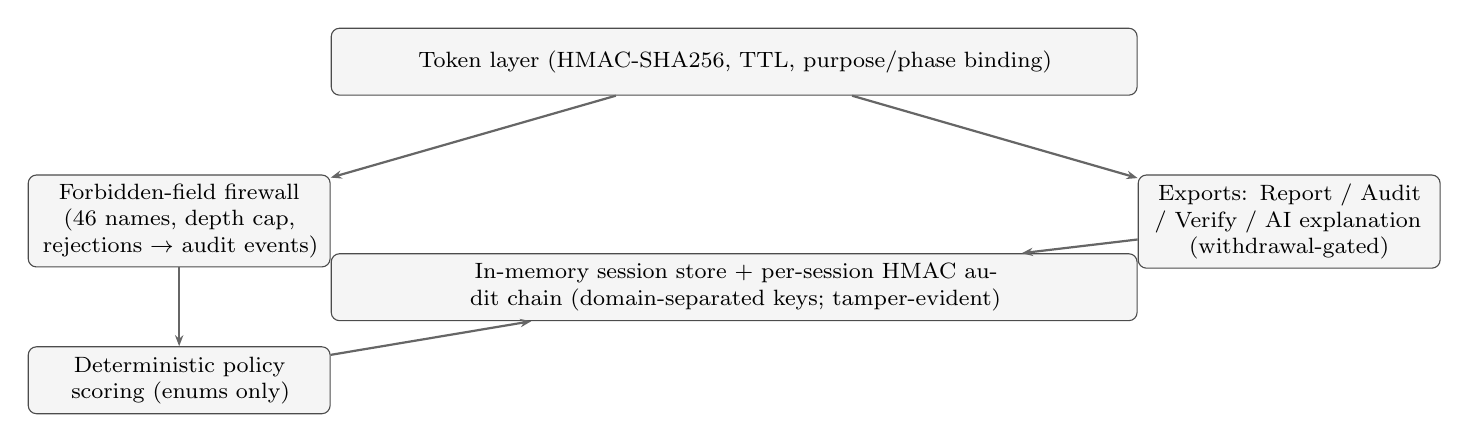
\begin{tikzpicture}[
  node distance=0.5cm and 0.7cm,
  box/.style={rectangle, rounded corners=3pt, draw=black!70, fill=gray!8,
              text width=3.6cm, align=center, font=\footnotesize,
              minimum height=0.85cm},
  arr/.style={-{Stealth[length=4pt]}, thick, black!60}
]
\node[box, text width=10cm] (token) {Token layer (HMAC-SHA256, TTL, purpose/phase binding)};
\node[box, below left=1.0cm and 0.0cm of token] (fw)
  {Forbidden-field firewall\\(46 names, depth cap, rejections $\rightarrow$ audit events)};
\node[box, below right=1.0cm and 0.0cm of token] (exp)
  {Exports: Report / Audit / Verify / AI explanation (withdrawal-gated)};
\node[box, below=1.0cm of fw] (policy) {Deterministic policy scoring (enums only)};
\node[box, below=2.0cm of token, text width=10cm] (store)
  {In-memory session store $+$ per-session HMAC audit chain (domain-separated keys; tamper-evident)};
\draw[arr] (token) -- (fw);
\draw[arr] (token) -- (exp);
\draw[arr] (fw) -- (policy);
\draw[arr] (policy) -- (store);
\draw[arr] (exp) -- (store);
\end{tikzpicture}
\caption{\sys{} architecture. Every write passes the forbidden-field firewall
before validation; every export is token-bound and chained. The system is
metadata-only by construction (C1).}
\label{fig:arch}
\end{figure*}

%% ── II. BACKGROUND ────────────────────────────────────────────────────────
\section{Background and Motivation}

A \sys{} session asks a participant to consent, complete one of five fictional
scenarios, and inspect exports: a Report, an Audit listing, a Verify check, and,
behind a default-off flag, an AI-style explanation (Fig.~\ref{fig:lifecycle}).
The scenarios resemble sensitive banking-adjacent moments: a mock data-sharing
consent screen, a mock payee-name check, a remote-access caution, a
payment-pause prompt, and an AI-agent finance approval. All scoring is a local
deterministic function over enumerated metadata. The labels safe/warning/critical
are fictional prototype outputs, not calibrated alerts.

Three observations from the project evidence shaped the design:

\begin{itemize}
  \item \textbf{O1.} Every prohibited input class the project tested (46 field
    names: credentials, OTPs, account identifiers, amounts, payees, device
    telemetry, and structural pollution keys) appeared only in attack-style
    tests. Each was rejected and logged. Refusal-as-evidence is therefore
    mechanically achievable within this prototype.
  \item \textbf{O2.} In the formative dry run, all five testers understood the
    non-claims (5/5 on fictional-only, no-bank-connection, no-fraud-detection,
    no-financial-advice, withdrawal), but only one of five initially understood
    the Report/Audit/Verify exports. Interpretability, not privacy, was the weak
    point. That result motivated the explanation layer and matches the broader
    finding that warning comprehension depends strongly on text characteristics
    and terminology~\cite{lindell2012protective,scherr2016text}.
  \item \textbf{O3.} The explanation layer is the riskiest place to improve
    interpretability because it sits at the boundary between internal evidence
    and reader-facing language. The design therefore treats the explanation
    layer as an adversarial surface, not a cosmetic feature.
\end{itemize}

\begin{figure}[t]
\centering
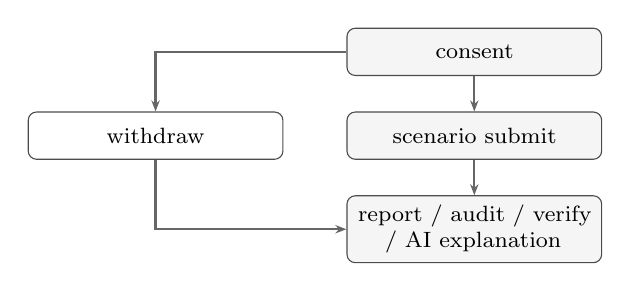
\begin{tikzpicture}[
  node distance=0.45cm,
  box/.style={rectangle, rounded corners=3pt, draw=black!70, fill=gray!8,
              text width=3.0cm, align=center, font=\footnotesize,
              minimum height=0.6cm},
  arr/.style={-{Stealth[length=4pt]}, thick, black!60},
  note/.style={font=\scriptsize, text=black!55, align=left}
]
\node[box] (consent) {consent};
\node[box, below=of consent] (submit) {scenario submit};
\node[box, below=of submit] (exports) {report / audit / verify / AI explanation};
\node[box, left=0.8cm of submit, fill=white] (withdraw) {withdraw};
\draw[arr] (consent) -- (submit);
\draw[arr] (submit) -- (exports);
\draw[arr] (consent) -| (withdraw);
\draw[arr] (withdraw) |- (exports);
\end{tikzpicture}
\caption{Session lifecycle. Withdrawal blocks report and explanation export
(403) but preserves audit/verify reads for transparency (C4).}
\label{fig:lifecycle}
\end{figure}

\begin{table}[t]
\caption{Allowed vs forbidden data (T1).}
\centering
\footnotesize
\begin{tabular}{p{3.7cm}p{3.7cm}}
\toprule
Allowed into the narrative payload (allowlist) & Forbidden everywhere
(46-name denylist, classes) \\
\midrule
Hashed session id & Credentials and one-time codes \\
Scenario type (enum) & Account/card/payment identifiers \\
User action/decision category (enum) & Amounts, balances, payees, references \\
Policy outcome $+$ score (deterministic) & Transaction/statement content \\
Manual-review flag (boolean) & Screens, recordings, keystrokes, clipboard \\
Privacy-assertion booleans & Window titles, process/app names, device ids \\
No free-text payload & \texttt{\_\_proto\_\_}, \texttt{prototype},
\texttt{constructor} \\
\bottomrule
\end{tabular}
\label{tab:data}
\end{table}

%% ── III. THREAT MODEL ─────────────────────────────────────────────────────
\section{Threat Model}

\textbf{Assets.} A1 sensitive banking payloads (must never enter); A2
audit-chain integrity; A3 the claim boundary; A4 participant anonymity; A5
official policy-result integrity.

\begin{table*}[t]
\caption{Threats and controls (T5).}
\centering
\footnotesize
\begin{tabular}{p{4.0cm}p{10.0cm}c}
\toprule
Threat & Controls & Asset \\
\midrule
T1 Sensitive/polluted submission & Recursive denylist firewall, depth cap, body
cap, rejection audit events, score escalation & A1 \\
T2 Provider exfiltration (future live LLM) & Allowlist input (hashed id, enums),
4\,KB cap, static no-egress gate, deterministic mock provider & A1 \\
T3 Capability overclaim in narrative & Output schema allowlist, length caps,
negation-aware claim scan, fail-closed rejection & A3 \\
T4 Narrative drifts official result & Equality check against the authoritative
record & A5 \\
T5 Audit-log tampering & Per-session HMAC chains, domain-separated keys;
tampered fixtures fail verification & A2 \\
T6 Token theft/replay & HMAC tokens, constant-time compare, TTL, purpose/phase
binding, path/token match & A1, A4 \\
T7 Withdrawal bypass & Withdrawn $\rightarrow$ 403 on report/explanation;
audit/verify intentionally readable & A4 \\
\bottomrule
\end{tabular}
\label{tab:threats}
\end{table*}

\noindent\textbf{Trust assumptions and residual risks.} The server, its secrets,
and transport security are trusted; Phase~B testers are trusted insiders. The
audit chain is tamper-evident, not tamper-proof: the server holds the keys, a
limitation shared by server-side secure-logging schemes generally, which
motivates third-party or distributed verification in that
literature~\cite{sree2019secure,ali2022bcals}. Denylist scanning is incomplete
by construction. Receipts attest process, not ground truth. Withdrawal does not
erase the metadata-only audit chain; the prototype discloses that choice. The
evaluation does not cover DoS beyond rate limiting, side channels, browser
compromise, or a malicious operator.

%% ── IV. DESIGN ────────────────────────────────────────────────────────────
\section{Design}

\sys{} uses the same rule at every boundary: construct what is allowed, reject
what is not, and record the rejection without recording the prohibited value.
The architecture applies that rule to submitted metadata, exports, explanation
inputs, explanation outputs, and participant withdrawal.

\subsection{Metadata-only integrity evidence (C1)}
\label{sec:c1}

Every write passes through a recursive forbidden-field firewall before schema
validation. The firewall blocks 46 key names spanning credentials, financial
identifiers, content fields, device telemetry, and the structural pollution keys
\texttt{\_\_proto\_\_}/\texttt{prototype}/\texttt{constructor}; it also enforces
a recursion-depth cap and a 16\,KB body limit. A rejection appends an audit
event containing the route, reason, and field name, never the value. The
session's later policy score escalates after a rejection, so an attack attempt
becomes part of the integrity record rather than a discarded exception. This
operationalises a data-minimisation design principle---in the limited
engineering sense of constructing only the metadata the stated prototype purpose
requires---as an enforced, evidence-producing mechanism rather than a policy
statement; we claim no regulatory compliance. The broader GDPR
data-protection-by-design context that motivates this posture is analysed in the
governance literature~\cite{klein2022pond,yeung2022demystifying}.
\emph{Alternative considered:} schema-level
allowlisting alone. The project rejected that as insufficient: an allowlist
validates shape, but it does not produce evidence of hostile attempts. \sys{}
therefore uses both controls. The allowlist defines the valid shape; the
denylist converts prohibited attempts into auditable signal.

\subsection{The deterministic AI privacy firewall (C2)}
\label{sec:c2}

\begin{figure*}[t]
\centering
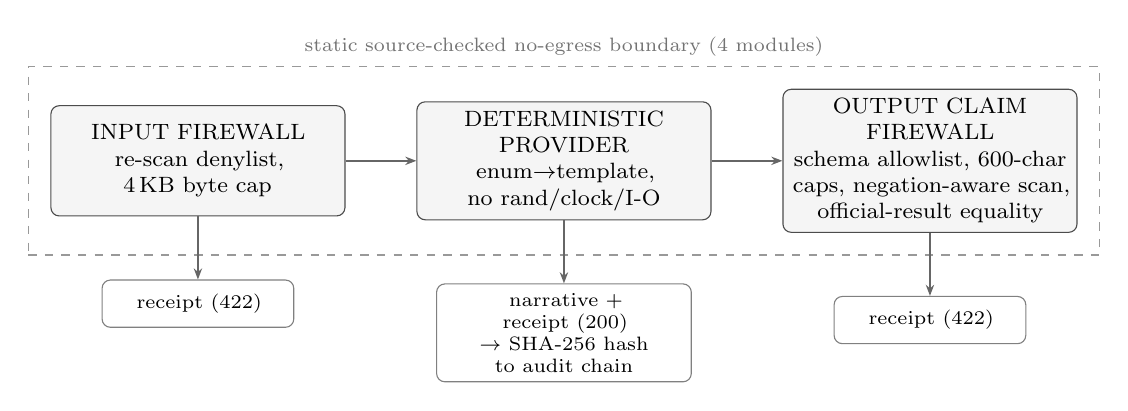
\begin{tikzpicture}[
  node distance=0.6cm and 0.9cm,
  stage/.style={rectangle, rounded corners=3pt, draw=black!70, fill=gray!8,
                text width=3.5cm, align=center, font=\footnotesize,
                minimum height=1.4cm},
  rcpt/.style={rectangle, rounded corners=3pt, draw=black!50, fill=white,
               text width=2.2cm, align=center, font=\scriptsize,
               minimum height=0.6cm},
  arr/.style={-{Stealth[length=4pt]}, thick, black!60}
]
\node[stage] (in) {INPUT FIREWALL\\re-scan denylist,\\4\,KB byte cap};
\node[stage, right=of in] (prov) {DETERMINISTIC PROVIDER\\enum$\rightarrow$template,\\no rand/clock/I-O};
\node[stage, right=of prov] (out) {OUTPUT CLAIM FIREWALL\\schema allowlist,
  600-char caps, negation-aware scan, official-result equality};
\node[rcpt, below=0.8cm of in] (r1) {receipt (422)};
\node[rcpt, below=0.8cm of out] (r2) {receipt (422)};
\node[rcpt, below=0.8cm of prov, text width=3.0cm] (ok)
  {narrative $+$ receipt (200)\\$\rightarrow$ SHA-256 hash to audit chain};
\node[draw=black!40, dashed, fit=(in)(prov)(out), inner sep=8pt,
      label={[font=\scriptsize,text=black!55]above:static source-checked
      no-egress boundary (4 modules)}] (boundary) {};
\draw[arr] (in) -- (prov);
\draw[arr] (prov) -- (out);
\draw[arr] (in) -- (r1);
\draw[arr] (out) -- (r2);
\draw[arr] (prov) -- (ok);
\end{tikzpicture}
\caption{The AI privacy firewall. The no-egress boundary is source-checked over
the four AI-firewall modules; every stage fails closed to a receipt, never to a
narrative (C2).}
\label{fig:firewall}
\end{figure*}

The explanation endpoint exists to make the report understandable without turning
the explanation layer into a privacy sink. We use ``AI-style'' to denote the
explanation-interface contract and guardrail pathway, not a live generative model
evaluated in this study. It therefore has four fail-closed stages:

\begin{enumerate}
  \item \textbf{Input firewall.} The narrative payload is \emph{constructed},
    not passed through: a hashed session id, scenario/action enums, the policy
    outcome, and the privacy-assertion booleans. The assembled payload is
    re-scanned against the forbidden-field denylist (defence in depth) and capped
    at 4\,KB. Failure returns a receipt, never a narrative.
  \item \textbf{Deterministic provider.} Narrative text is an enum-to-template
    pure function: no randomness, no clock, no I/O. A static source gate checks
    that the four AI-firewall modules import no network primitive, and a negative
    self-test confirms the gate fails when a network primitive is injected. This
    is not a host-level egress-control claim.
  \item \textbf{Output claim firewall.} The narrative must match an exact
    top-level schema (field allowlist), respect 600-character caps per field,
    contain a non-empty non-claims list, and pass a negation-aware scan over 29
    affirmative-capability phrasings; an equality check proves the narrative did
    not drift the official result.
  \item \textbf{Privacy receipt.} Every response, whether successful, blocked, or
    disabled, carries a receipt: provider identity
    (\texttt{deterministic\_mock}), \texttt{sensitive\_payload\_sent\_to\_ai:false},
    \texttt{network\_egress\_used:false}, official-result and claim-guard flags,
    and a success-only SHA-256 narrative hash that is also written into the
    session's audit chain.
\end{enumerate}

\emph{Alternative considered:} a live LLM behind the same firewall. The project
rejected it for this paper because it would convert the no-egress property from
static source evidence into an operational assertion. The input allowlist, byte
cap, output schema, claim scan, and receipt mechanism would survive a future
live provider. Determinism and reproducible narrative hashing would not; a live
provider would require replay logging and separate provider-risk evaluation. The
mock therefore establishes the contract and enforcement points, not live-model
safety.

\subsection{Claim discipline as a mechanism (C3)}
\label{sec:c3}

The output firewall's scanner is negation-aware. Required disclaimers such as
``not fraud detection'' and ``not a fraud detection tool'' pass; affirmative
phrasing and weakened negation such as ``not really a \ldots'' are blocked. The
scanner is intentionally conservative: a false positive blocks a narrative, and
the paper claims no complete false-negative class. Repository CI enforces the
same boundary with an overclaim-wording scanner. During integration, that scanner
flagged the firewall's own denylist because the denylist contains the phrases it
blocks. The project resolved the conflict with an explicit scanner exclusion
rather than string obfuscation. Claim discipline is therefore checked at runtime
and again at repository level.

\subsection{Verifiable participation lifecycle (C4)}
\label{sec:c4}

Each session carries an HMAC-SHA256 audit chain with domain-separated keys:
participant-code hashing and chain signing cannot be cross-validated.
Participants can export a Report, an Audit listing, and a Verify check of chain
consistency. The Report contains explicit privacy assertions; the sensitive-data
assertions remain \texttt{false} when the firewall has blocked prohibited input.
Withdrawal blocks Report and explanation export, but keeps Audit and Verify
readable so a participant can still inspect the chain. The human-evidence pipeline
stores only aggregate counts.

\begin{table}[t]
\caption{Claims vs non-claims (T4).}
\centering
\footnotesize
\begin{tabular}{p{3.7cm}p{3.7cm}}
\toprule
The paper claims & The paper does NOT claim \\
\midrule
Metadata-only integrity evidence (about the process) & Fraud detection or scam
prevention \\
A fictional banking-adjacent prototype & Real banking protection or payment
safety \\
A trusted internal dry run (formative) & Real payee verification or financial
advice \\
A deterministic AI privacy firewall (contract $+$ gates) & CDR/APRA/AML/CTF
compliance \\
AI-style explanation without sensitive payloads & Production readiness or
bank-grade security \\
\bottomrule
\end{tabular}
\label{tab:claims}
\end{table}

%% ── V. IMPLEMENTATION ─────────────────────────────────────────────────────
\section{Implementation}

The implementation uses Node.js/Express, static HTML/CSS/JS tester pages, an
in-memory session store, and shell/Node CI gates. The explanation panel writes
through \texttt{textContent} only. The explanation endpoint sits behind a
default-off flag requiring the exact string \texttt{"true"}; requests must be
token-bound, path-matched, and within the read-rate limit. The prototype is
single-node and research-only.

%% ── VI. EVALUATION ────────────────────────────────────────────────────────
\section{Evaluation}

The evaluation is bounded by the prototype's research-only scope. It asks three
questions:
\begin{itemize}
  \item \textbf{E1.} Do the structural controls pass their automated gates?
  \item \textbf{E2.} Can trusted insiders complete the lifecycle and understand
    the prototype's non-claims?
  \item \textbf{E3.} Does the explanation firewall pass a clean narrative and
    block a poisoned one?
\end{itemize}

\subsection{Gate results (E1)}

\emph{Hypothesis:} the prototype's claimed structural properties can be checked
mechanically. \emph{Result:} at the evidence freeze, every automated gate passed
(Table~\ref{tab:gates}). The claim is deliberately narrow: the gates passed for
the frozen prototype and evidence pack. The result does not establish production
security or regulatory compliance.

\begin{table}[t]
\caption{Gate results at evidence freeze (T3).}
\centering
\footnotesize
\begin{tabular}{ll}
\toprule
Gate & Result \\
\midrule
Unit tests & 417/417 pass \\
Banking smoke & 14/14 pass \\
AI firewall smoke & 5/5 pass \\
Full banking E2E smoke & 43/43 pass (incl.\ tamper-evidence check) \\
Banking security audit & 27/27 pass \\
Banking privacy audits & all 3 PASS \\
No-egress static gate & PASS (with negative self-test) \\
Dependency audit & 0 vulnerabilities \\
Repository CI quality gate & green \\
\bottomrule
\end{tabular}
\label{tab:gates}
\end{table}

\subsection{Formative internal dry run (E2, exploratory)}
\label{sec:dryrun}

\emph{Hypothesis:} trusted insiders can complete the lifecycle and understand
the non-claim checklist. \emph{Result:} five trusted internal testers completed
30 sessions (Table~\ref{tab:phaseb}). No tester entered real banking values; the
evidence pack contained zero sensitive values; the deterministic policy pattern
reproduced identically across testers (safe/warning/warning/warning/safe across
the five scenario types); all five withdrawals blocked later report export; and
all five testers passed the five-item non-claim checklist. The weak point was
export interpretability: only 1/5 initially understood the Report/Audit/Verify
exports. A focused 3-session rerun confirmed revised copy, but it cannot
establish improvement; we report it only as a design iteration. This is a
formative dry run with $n=5$ trusted insiders, not a user study and not a
representative banking-customer sample.

\begin{table}[t]
\caption{Phase~B aggregates (T2, exploratory).}
\centering
\footnotesize
\begin{tabular}{lr}
\toprule
Measure & Value \\
\midrule
Trusted internal testers & 5 \\
Total sessions & 30 \\
Submitted scenario sessions & 25 (5 per scenario) \\
Withdrawal sessions & 5 \\
Withdrawals blocking later report export & 5/5 \\
Real banking values entered & 0 \\
Sensitive values found in evidence & 0 \\
Forbidden payload structures in evidence & 0 \\
Comprehension: fictional-only & 5/5 \\
Comprehension: no bank connection & 5/5 \\
Comprehension: no fraud detection & 5/5 \\
Comprehension: no financial advice & 5/5 \\
Comprehension: withdrawal & 5/5 \\
Export interpretability (pre copy-patch) & 1/5 \\
\bottomrule
\end{tabular}
\label{tab:phaseb}
\end{table}

\subsection{Fixture studies (E3)}

\emph{Hypothesis:} the output firewall passes a clean narrative and blocks a
poisoned one. \emph{Result:} the accepted-explanation fixture, a clean generated
narrative with receipt, passes all gates and contains no attack values. The
rejected-claim fixture, a deliberately poisoned narrative asserting a detection
capability, is blocked by the claim guard with the failed gate recorded in its
receipt. The fixture pair demonstrates the firewall's two required behaviours
under controlled conditions.

%% ── VII. LIMITATIONS ──────────────────────────────────────────────────────
\section{Limitations}

The strongest limitation is also the point of the paper: the provider is a
deterministic mock. No live LLM has been filtered, evaluated, or validated. The
mock lets the paper isolate the contract around an explanation provider, but it
does not measure real model behaviour.

The human evidence is formative. Five trusted insiders completed the dry run; the
paper makes no statistical claim, no representative-user claim, and no
banking-customer comprehension claim. The result supports lifecycle feasibility
and checklist comprehension within a trusted internal setting.

The security evidence is bounded. Denylist scanning is incomplete by
construction, and adversarial phrasing can evade a phrase scanner. The allowlist
construction is the stronger control. The gates are written by the project they
validate; negative self-tests and public reproducibility reduce that risk but do
not remove it. The prototype is single-node and in-memory. The audit chain is
server-keyed, tamper-evident to participants, not tamper-proof against the
operator. The no-egress claim is a static source check over the four AI-firewall
modules, not a network sandbox or host-level egress-control guarantee.

%% ── VIII. REPRODUCIBILITY ─────────────────────────────────────────────────
\section{Reproducibility and Review-Substitute Pack}

The artifact includes the paper, evidence pack, final audit, claim audit, and
Stage~B5-R review-substitute pack under \texttt{papers/banking-shield/} and
\texttt{docs/research/banking-pilot/}. The Stage~B5-R pack simulates five
external-style hostile reviews (privacy/security, banking governance, HCI, AI
safety, and reject-oriented reviewer~\#2 attack) and records author responses
before preprint submission. This is not a replacement for formal peer review; it
is a structured preprint-risk-reduction step. The core reproduction gates are:

{\scriptsize
\begin{verbatim}
npm test
bash scripts/smoke-banking-pilot.sh
SIMURGH_BANKING_PILOT_AI_EXPLAIN=true \
  bash scripts/smoke-banking-pilot-ai-firewall.sh
bash scripts/smoke-banking-pilot-full-e2e.sh
bash scripts/security-audit-banking-pilot.sh
node scripts/privacy-audit-banking-pilot.mjs
node scripts/privacy-audit-banking-pilot-phase-b.mjs
node scripts/privacy-audit-banking-pilot-ai-firewall.mjs
npm audit --audit-level=moderate
\end{verbatim}
}

\noindent These gates support the paper's mechanism and evidence-pack claims.
They do not establish production security, regulatory compliance, live-LLM
safety, or real-world banking effectiveness.

%% ── IX. RELATED WORK ──────────────────────────────────────────────────────
\section{Related Work}

\textbf{Tamper-evident logging.} Secure-logging schemes protect log integrity
and authenticity with hash chains, MACs, and related structures, and survey the
limits of server-trusted designs~\cite{sree2019secure,ali2022bcals}. We apply
standard HMAC-chain machinery per-session, with participant-facing verify exports
and withdrawal semantics; our chain is deliberately scoped as tamper-evident, not
tamper-proof.

\textbf{Warning and rights comprehension.} Warning research shows comprehension
hinges on reception, attention, and terminology~\cite{lindell2012protective},
that recipients frequently take no action on textual alerts~\cite{kim2019wireless},
and that text characteristics measurably drive comprehension of rights-style
warnings~\cite{scherr2016text}. \sys{} measures comprehension of \emph{non-claims}
---what the system does NOT do---as an inverted warning problem, in a formative
setting only.

\textbf{Data minimisation and design-based regulation.} The GDPR's
data-minimisation and data-protection-by-design principles require systems to
hold only what their purpose strictly needs and to hard-wire protection into
architecture~\cite{klein2022pond,yeung2022demystifying,bradshaw2019privacy}. Our
firewall is one concrete design-based mechanism, with the additional property
that refusals produce evidence; we claim no compliance status under any
regulation.

\textbf{LLM guardrails and AI risk frameworks.} A growing literature examines
bias and risk across the life cycle of large language models~\cite{lee2024lifecycle}
and catalogues AI trust, risk, and security management (TRiSM) controls,
including runtime enforcement and output filtering~\cite{ray2026trism}. Such
approaches typically filter or monitor content emitted by a live model; \sys{}
instead makes the provider structurally unable to receive sensitive input,
statically unable to egress, and schema-bound on output, with content scanning
only as the final layer.

\textbf{Open-banking consent UX.} Open-banking customer-experience guidance
treats consent and access dashboards as critical user-control
surfaces~\cite{openbanking_consent,worldbank_consent}. \sys{} does not evaluate
real open-banking consent efficacy; it evidences the integrity of a fictional
consent-style flow.

\textbf{Payee-confirmation services.} Confirmation-of-payee and
verification-of-payee schemes perform account-name matching before payment
initiation~\cite{payuk_cop,epc_vop}. \sys{}'s payee scenario is fictional: the
contribution is the metadata boundary, not name matching.

\textbf{Per-response AI transparency artifacts.} Model cards and datasheets
document models or datasets as release-time
artifacts~\cite{mitchell2019modelcards,gebru2021datasheets}. \sys{}'s receipts
are narrower: per-response, machine-checked records of what the explanation
pipeline did and did not receive.

%% ── X. CONCLUSION ─────────────────────────────────────────────────────────
\section{Conclusion}

\sys{} asks a narrow systems question with practical consequences: can a sensitive
research prototype add an explanation layer while preserving machine-checkable
boundaries around data collection, provider input, network egress, and
reader-facing capability claims? The prototype's answer is a structural pattern:
fail-closed metadata firewalls, a deterministic offline provider behind
provider-independent enforcement points, machine-checked claim discipline, and
per-response receipts anchored in tamper-evident audit chains. At the evidence
freeze, every automated gate passed. In a formative five-tester dry run,
participants completed the lifecycle, the evidence pack contained zero sensitive
values, and all testers understood the non-claim checklist.

The contribution is not banking protection and not live-LLM validation. It is a
reproducible way to make absence claims inspectable: show what the system was
allowed to construct, show what it rejected, show what the explanation provider
received, and show what the output firewall would not let the system say. Future
work should test the same contract with replay-logged live-provider integration,
generated allowlist templates, externally countersigned receipts, independent
security review, and a powered user study.

%% ── XI. LLM DISCLOSURE ────────────────────────────────────────────────────
\section{LLM-Assistance Disclosure}
\label{sec:llm}

This paper was drafted with substantial assistance from a frontier language model
operating under a logged, evidence-pack-constrained protocol: the model
synthesised, critiqued, and drafted; it validated nothing. A second
model-assisted independent-style review stage simulated five hostile reviewer
roles and produced an author response before this preprint candidate. All factual
statements trace to automated gate results, generated fixtures, frozen aggregate
evidence, and explicit audit records. Citation candidates were verified against
CrossRef metadata before inclusion; unresolved placeholders are not retained in
this version.

%% ── REFERENCES ────────────────────────────────────────────────────────────
\bibliographystyle{IEEEtran}
\bibliography{references}

\end{document}
